\documentclass[tikz,border=30mm]{standalone}
\input{prbl.tex}
\usepackage{amsmath, amsfonts}

%defining new colors : 

\definecolor{eblue}{HTML}{00FFF6}
\definecolor{eblack}{HTML}{212529}
\definecolor{emauve}{HTML}{3D0043}
\definecolor{eviolet}{HTML}{E11D74}
\definecolor{egreen}{HTML}{91D18B}
\definecolor{egray}{HTML}{E9E8E8}
\definecolor{epink}{HTML}{FFABE1}
\definecolor{violet1}{HTML}{937DC2}
\definecolor{violet2}{HTML}{F70776}
\definecolor{violet3}{HTML}{EA21A2}



\begin{document}
\pagecolor{emauve!50!black}

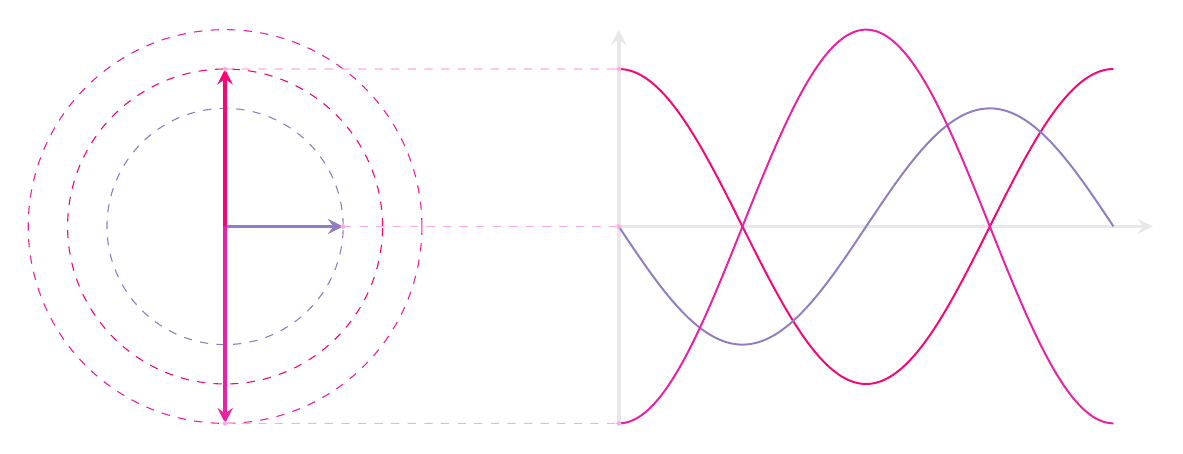
\begin{tikzpicture}[>=stealth]

%the dashed circles
\draw[dashed, violet1] (0,0)circle(1.5);
\draw[dashed, violet2] (0,0)circle(2); 
\draw[dashed, violet3] (0,0)circle(2.5); 

%the vectors associated to the sinusoidal functions
\draw[line width=0.5mm, ->, violet1] (0,0)--(0:1.5);
\draw[line width=0.5mm, ->, violet2] (0,0)--(90:2);
\draw[line width=0.5mm, ->, violet3] (0,0)--(-90:2.5);

\begin{scope}[shift={(5,0)}]
%x and y axis
\draw[line width = 0.5mm, egray, ->] (0,-2.5)--(0,2.5);
\draw[line width = 0.5mm, egray, ->] (0,0)--(2*pi+0.5,0);

%The sine functions with different phases 
\draw[line width=0.25mm, violet2, samples=300, variable=\t, domain=0:2*pi] plot(\t, {2*sin((\t + (90*pi/180)) r)});

\draw[line width=0.25mm, violet1, samples=300, variable=\t, domain=0:2*pi] plot(\t, {-1.5*sin((\t + (0*pi/180)) r)});

\draw[line width=0.25mm, violet3, samples=300, variable=\t, domain=0:2*pi] plot(\t, {-2.5*sin((\t + (90*pi/180)) r)});

%marking the (0,f(0)) nodes 
\coordinate(sin1) at (0,{2*sin((90*pi/180) r)});
\coordinate(sin2) at (0,{-1.5*sin((0*pi/180) r)});
\coordinate(sin3) at (0,{-2.5*sin((90*pi/180) r)});
\end{scope}

%arking the tip of the arrows
\coordinate(vec1) at (90:2);
\coordinate(vec2) at (0:1.5);
\coordinate(vec3) at (-90:2.5);

\filldraw[epink] (vec1)circle(0.025);
\filldraw[epink] (sin1)circle(0.025);
\draw[dashed, epink] (vec1)--(sin1);

\filldraw[epink] (vec2)circle(0.025);
\filldraw[epink] (sin2)circle(0.025);
\draw[dashed, epink] (vec2)--(sin2);

\filldraw[epink] (vec3)circle(0.025);
\filldraw[epink] (sin3)circle(0.025);
\draw[dashed, epink] (vec3)--(sin3);


\end{tikzpicture}

%To obtain the animated version you can loop through the angles with a foreach loop, it's simple give it a shot ;) 

\end{document}
